\documentclass{article}
\usepackage[T1]{fontenc}
\usepackage{lmodern}
\usepackage[spanish,es-noshorthands]{babel}
\usepackage{float}
\usepackage{graphicx} % Required for inserting images
\usepackage{amsmath}  % \substack y \text en las ecuaciones
\renewcommand{\contentsname}{Índice}
\begin{document}
\begin{figure}
    \centering
    
\includegraphics[width=0.3\linewidth]{logo_tecnun.png}
    \label{fig:placeholder}
\end{figure}
\vspace{2cm}
\title{TECNUN, UNIVERSIDAD DE NAVARRA\\[4cm] MODELO DE OPTIMIZACIÓN: PLANIFICACIÓN ACADÉMICA Y DEPORTIVA }
\author{Beñat Ilzarbe Daza \\ Aitor Marcalain Mauleon}
\date{Abril 2026}

\maketitle
\newpage
{\renewcommand{\baselinestretch}{1.5}\selectfont
\tableofcontents
}
\newpage
\section{Descripción del proyecto}

Este proyecto surge de una situación bastante común en el ámbito académico: la dificultad para gestionar adecuadamente el tiempo. Cuando la carga de trabajo es elevada, la planificación manual no siempre resulta eficaz, lo que puede derivar en la acumulación de tareas, picos de estrés o incluso en procrastinación involuntaria.
\vspace{0.5cm}

Desde otro punto de vista, este problema puede interpretarse de forma similar a uno de logística. Se dispone de una serie de tareas, como los exámenes, cada una con unas necesidades concretas de horas de estudio, y de un recurso limitado, que es el tiempo disponible. El objetivo no es únicamente cumplir con todas ellas, sino hacerlo de la forma más equilibrada posible, evitando sobrecargas y reduciendo el estrés a lo largo del proceso.

\vspace{0.5cm}

Este modelo debe determinar de forma automática cómo repartir las horas diarias entre las distintas asignaturas y la actividad física, cumpliendo los siguientes requisitos:

\begin{itemize}
    \item Cubrir el total de horas de estudio necesarias para múltiples asignaturas.
    \item Garantizar un refuerzo final de estudio en los días previos a cada examen.
    \item Mantener una rutina mínima de actividad física como mecanismo de regulación del estrés.
\end{itemize}

\section{Modelo matemático}

El problema se ha planteado como un modelo de optimización lineal entera mixta, ya que combina decisiones continuas (horas) con decisiones binarias (realizar o no una actividad).

\subsection{Variables de entrada}

Para poder ejecutar el modelo, se consideran los siguientes datos de partida:

\begin{itemize}
    \item $A$: conjunto de asignaturas, cada una con una carga de trabajo asociada.
    \item $D$: horizonte temporal de planificación (días disponibles).
    \item $Capacidad_d$: número máximo de horas disponibles cada día $d$.
    \item $D_a$: día en el que tiene lugar el examen de la asignatura $a$.
\end{itemize}

\subsection{Variables de decisión}

El problema se ha modelado utilizando un total de $N$ variables de decisión, donde:

\[
N = 2 \cdot D \cdot A + 3 \cdot D
\]

Las variables se dividen en los siguientes grupos:

\begin{itemize}
    \item $x_{a,d}$: horas de estudio de la asignatura $a$ en el día $d$ (variable continua).
    \item $y_{a,d}$: variable binaria que indica si se estudia la asignatura $a$ el día $d$.
    \item $e_d$: horas dedicadas al deporte en el día $d$ (variable continua).
    \item $z_d$: variable binaria que indica si se realiza deporte el día $d$.
    \item $r_d$: horas de descanso o tiempo libre en el día $d$ (variable continua).
\end{itemize}

\subsection{Función objetivo}

El modelo busca minimizar el estrés total acumulado, penalizando especialmente las horas de estudio cercanas a los exámenes y favoreciendo tanto el deporte como el descanso. La función objetivo es:

\[
\min Z = \sum_{a=1}^{n_A} \sum_{d=1}^{n_D} \left( W_{a,d} \cdot x_{a,d} \right) 
- \sum_{d=1}^{n_D} \left( \beta \cdot e_d + \gamma \cdot r_d \right)
\]

En cuanto al peso académico $W_{a,d}$, su valor es dinámico de forma que cambia en función de la cercanía al examen:

\[
W_{a,d} = 1 + \frac{\alpha}{(D_{exam,a} - d) + 1}
\]

De esta forma, se evita concentrar todo el estudio en los últimos días.

\subsection{Restricciones del modelo}

Siguiendo la formulación de la programación lineal entera mixta, se han definido las siguientes restricciones:

\paragraph{A. Carga lectiva total}

Para cada asignatura, se garantiza que se cumplen las horas necesarias antes del examen:

\[
\sum_{d=1}^{D_{exam,a}-1} x_{a,d} \geq horas_a, 
\quad \forall a \in \{1, \dots, n_A\}
\]

\paragraph{B. Capacidad diaria}
Se utiliza la variable de descanso para no superar el tiempo disponible cada día:

\[
\sum_{a=1}^{nA} x_{a,d} + e_d + r_d \leq Capacidad_d, 
\quad \forall d \in \{1, \dots, nD\}
\]

\paragraph{C. Lógica de bloques mínimos y máximos}

Para evitar sesiones irreales, se imponen límites mínimos y máximos vinculados a variables binarias:

\begin{itemize}
    \item Estudio:
    \[
    min\_est \cdot y_{a,d} \leq x_{a,d} \leq max\_est \cdot y_{a,d}
    \]
    \item Deporte:
    \[
    min\_dep \cdot z_d \leq e_d \leq max\_dep \cdot z_d
    \]
\end{itemize}

\paragraph{D. Requisitos de salud y rendimiento}\mbox{}\\

\textit{Mínimo semanal de deporte:}

\[
\sum_{d=d_i}^{d_f} e_d \geq min\_dep\_sem \cdot \frac{\text{días\_semana}}{7}
\]

\textit{Sprint final académico:}

\[
\sum_{\substack{d = D_{\mathrm{exam},a} \\ - \mathrm{sprint\_dias}}}^{D_{\mathrm{exam},a} - 1} x_{a,d} \geq \mathrm{sprint\_horas}
\]

\paragraph{E. Coherencia temporal}

No se permite asignar horas de estudio una vez pasado el examen:

\[
x_{a,d} = 0, \quad y_{a,d} = 0 
\quad \forall d \geq D_{exam,a}
\]

\subsection{Implementación en Matlab (CPLEX)}

La implementación se ha realizado mediante una función que construye el modelo organizando el vector de costes ($f$), el tipo de cada variable (\texttt{ctype}) y las matrices de restricciones ($A$ y $b$).
Para adaptar el problema al formato de CPLEX, se ha utilizado un sistema de indexación lineal que permite representar todas las variables en un único vector.
\vspace{0.5cm}

Además, se han incorporado distintos interruptores lógicos (como \texttt{debug\_sprint} o \texttt{debug\_deporte\_semanal}) que permiten activar o desactivar ciertas restricciones. Esto facilita analizar cómo afectan al resultado.

\section{Proceso de construcción del programa y problemas afrontados}

Hemos decidido añadir esta sección dado que el programa no compilaba en un principio, la salida de \textit{cyplex.solve()} era infeasible. Tras repasar bien los parametros con los que modelabamos el programa nos dimos cuenta de un problema muy claro: la capacidad diaria (en horas) no era suficiente para cubrir todas las exigidas por cada asignatura, teniendo que cumplir un mínimo de deporte a la semana.

\vspace{0.5cm}

Esta realización se nos ocurrio despues de un proceso de desactivación de algunas de nuestras restricciones. Al poner el booleano \texttt{debug\_deporte\_semanal = False} el problema compilaba y encontraba solución optima, por lo que el problema se concentraba en esa restricción.

\vspace{0.5cm}

Una primera idea fue reducir el parámetro de deporte semanal para que fuese mas probable que se encontrase una solución cumpliendo su restricción asociada. Aun así, el problema seguía siendo que la suma de capacidad diaria era muy cercana a el total de horas necesitadas para estudiar. 

\vspace{0.5cm}

Entonces, aumentemos la capacidad diaria para estudiar y hacer deporte en dos horas diarias, lo cual estando en epóca de examenes nos pareció coherente y realista. Así, obtuvimos la primera solución y pudimos proceder a experimentar con el modelo. 

\section{Experimentos y análisis de resultados}

En esta sección se presentan los resultados obtenidos al aplicar el modelo de optimización sobre distintos escenarios. El objetivo es validar que el algoritmo no solo encuentra soluciones factibles, sino que estas son lógicas y se adaptan a las variaciones en los parámetros de entrada.


\subsection{Experimento I: Horizonte de 8 semanas y 6 asignaturas}

Este primer experimento se utiliza como base para testear la robustez del modelo. Sobre una estructura fija de 56 días y 6 asignaturas, se han introducido variaciones en los pesos de la función objetivo y en las exigencias de las restricciones para observar la respuesta del sistema.

\subsubsection{Validación de la distribución y coherencia temporal}

En las pruebas iniciales se confirma que el modelo gestiona correctamente la carga de estudio total por asignatura (3 asignaturas de 30h y 3 de 50h). Se observa cómo se adelanta el estudio de las asignaturas con exámenes más tardíos cuando existe disponibilidad, asegurando que el ``vaciado'' de horas de cada materia coincida exactamente con su fecha de examen.

\begin{figure}[H]
    \centering
    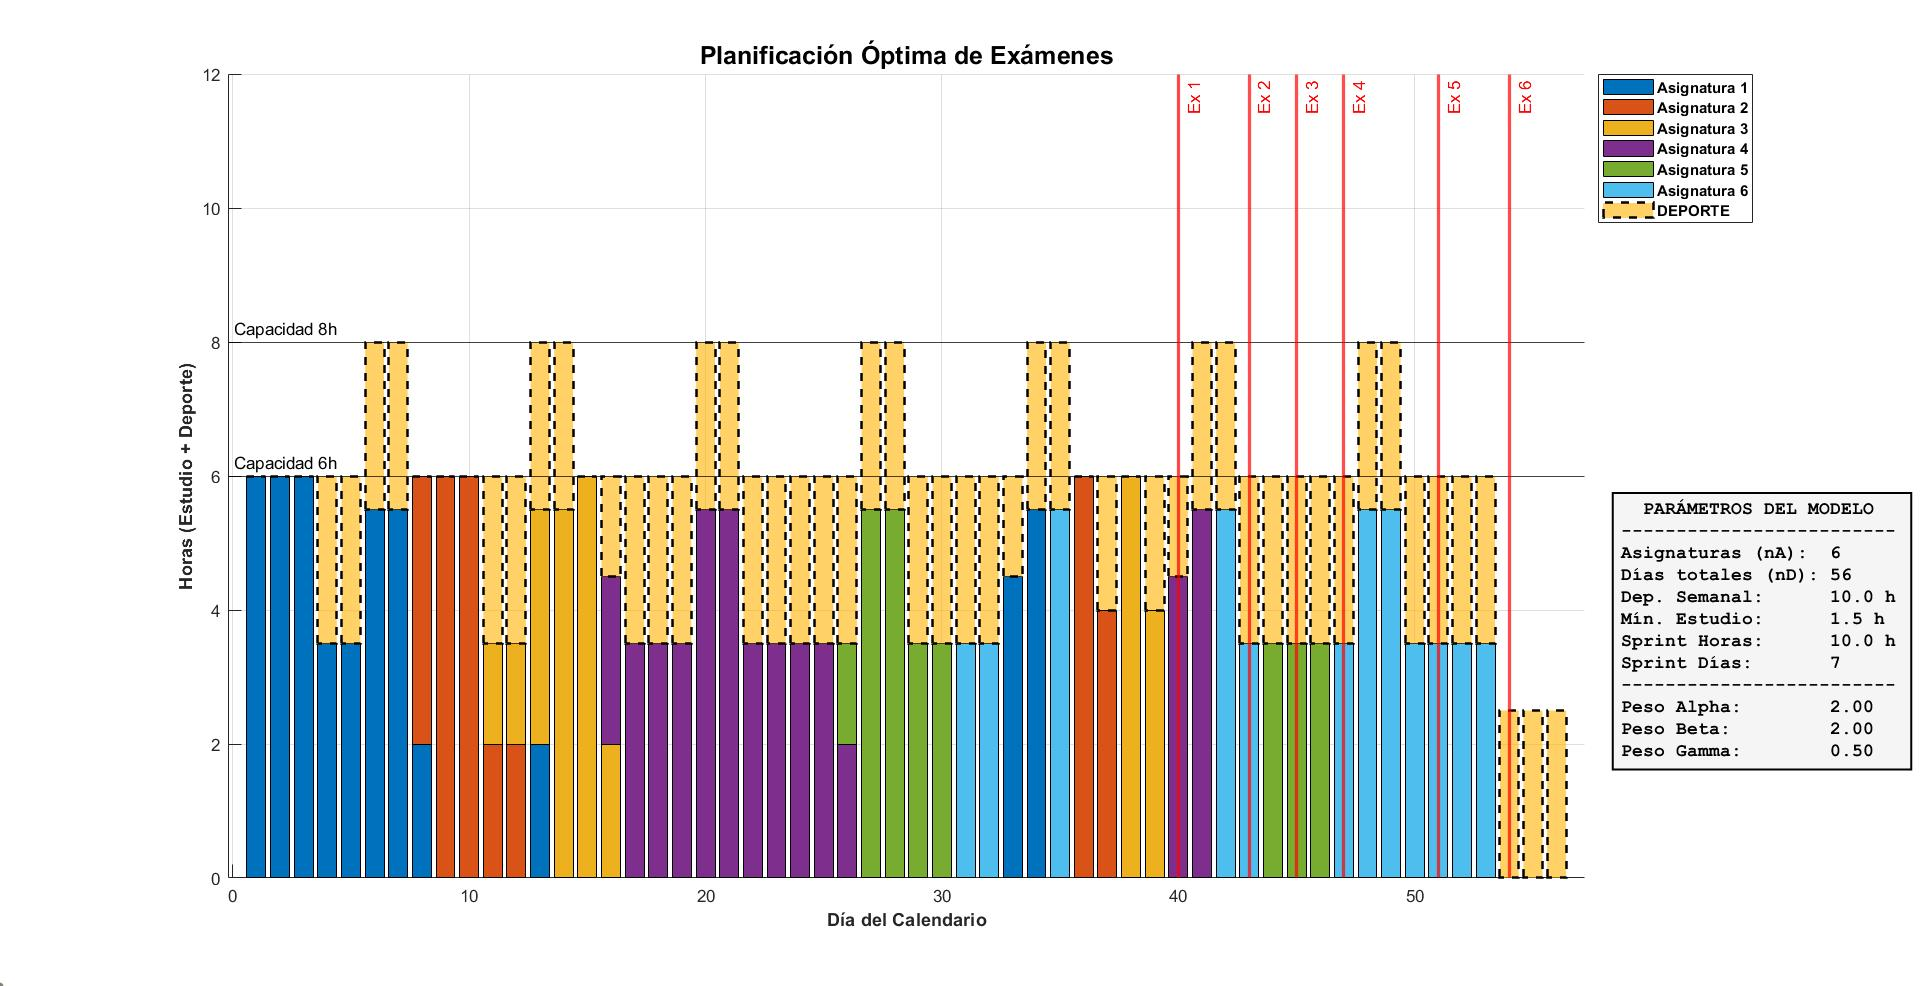
\includegraphics[width=0.75\linewidth]{FIGURA_1.jpg}
    \caption{Calendario académico balanceado}
    \label{fig:placeholder}
\end{figure}

La restricción de sprint final se cumple estrictamente, generando picos de actividad controlados que no superan la capacidad diaria establecida.

\begin{figure}[H]
    \centering
    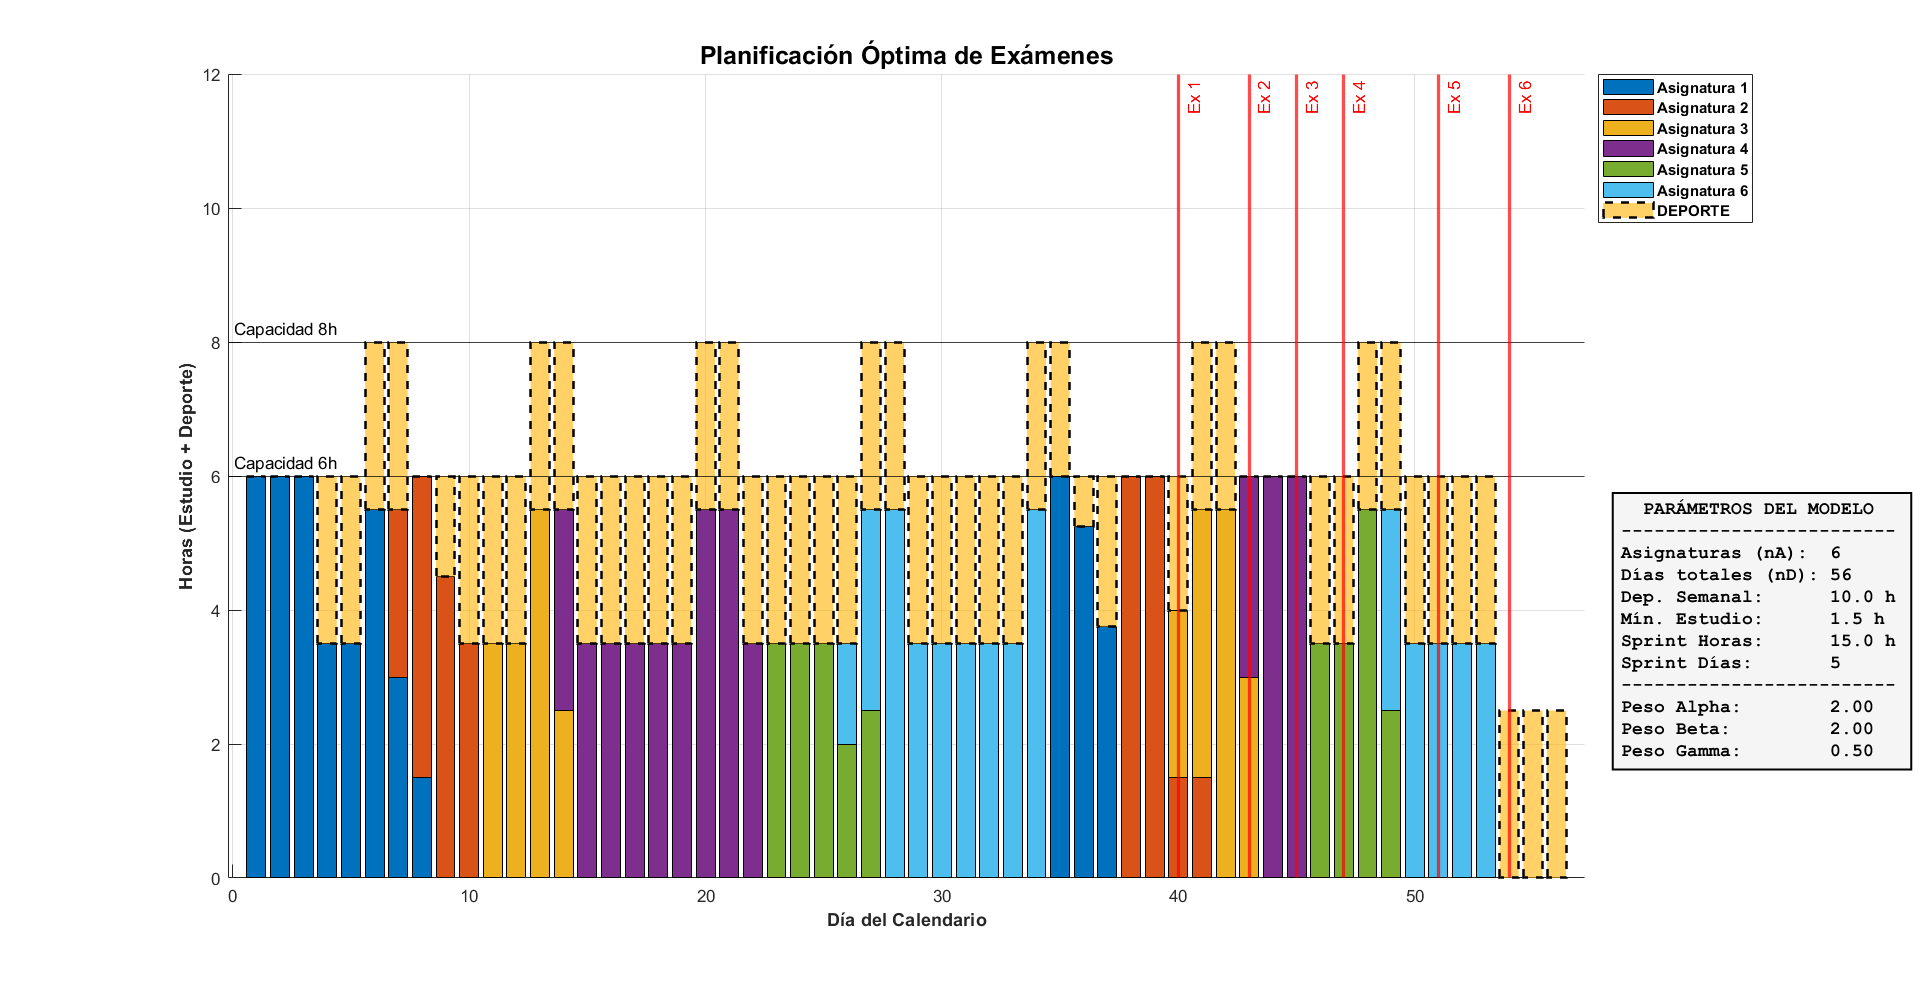
\includegraphics[width=0.75\linewidth]{FIGURA_4.png}
    \caption{Calendario académico con gran sprint final}
    \label{fig:placeholder}
\end{figure}

\subsubsection{Sensibilidad a los factores de bienestar (Deporte y Descanso)}

Manteniendo el mismo calendario de exámenes, se han ajustado los coeficientes $\beta$ (deporte) y $\gamma$ (descanso) para evaluar la flexibilidad de la planificación:

\begin{itemize}
    \item \textbf{Priorización del ejercicio:} Al haber mantenido durante todas las pruebas el peso del deporte $\beta$ por encima del peso del descanso $\gamma$, el tiempo que había libre de estudio se ha rellenado con horas de deporte, tal y como hemos visto en los experimentos anteriores.

    \item \textbf{Maximización del descanso:} En configuraciones donde se prima el descanso, el modelo tiende a agrupar el estudio en bloques más densos para liberar días completos de inactividad, especialmente en las semanas alejadas de los exámenes donde el coste de oportunidad del tiempo es menor.

    \begin{figure}[H]
        \centering
        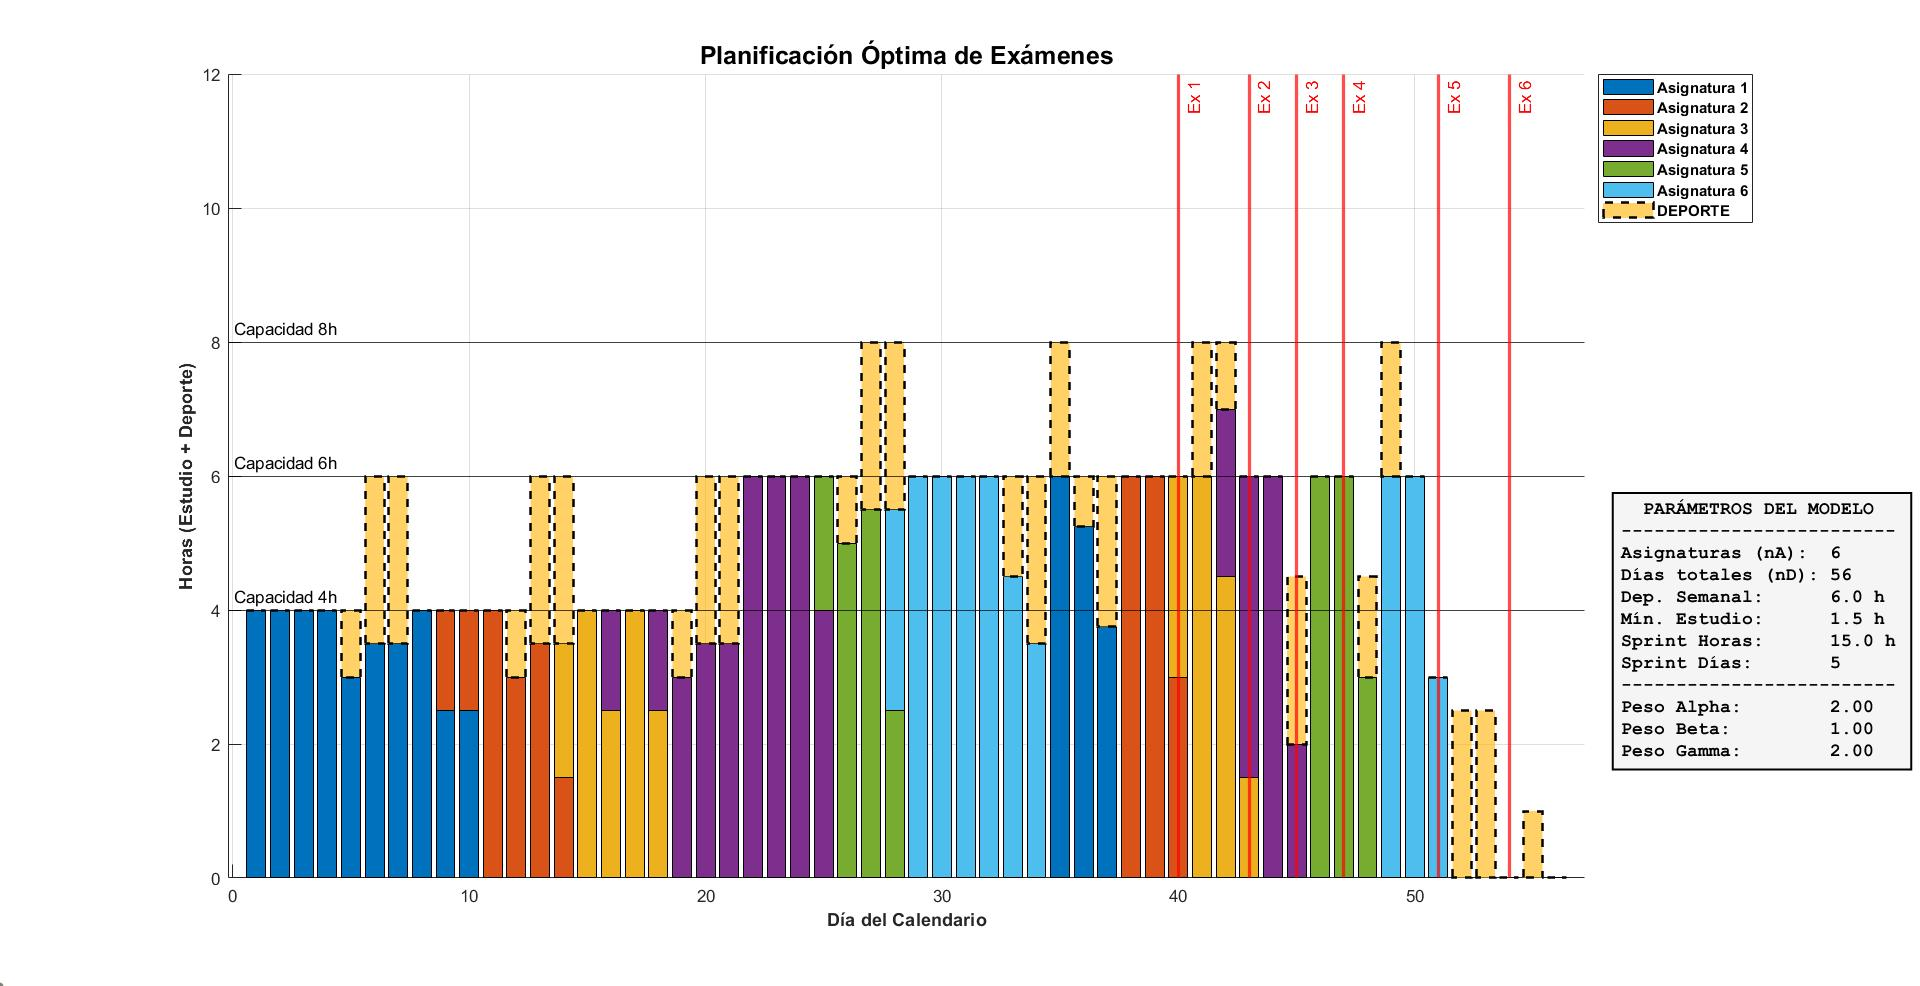
\includegraphics[width=0.75\linewidth]{FIGURE_5.jpg}
        \caption{Calendario académico; maximización del descanso}
        \label{fig:placeholder}
    \end{figure}

    \item \textbf{Gestión de la saturación del descanso:}
    En este escenario, se ha aplicado un valor muy elevado al coeficiente de descanso ($\gamma$) con el objetivo de intentar saturar el modelo y ver su reacción en un caso extremo de sedentarismo. A pesar de la alta densidad de exámenes en las semanas finales, el modelo demuestra su capacidad para encontrar una solución que preserve periodos de inactividad.

    \begin{figure}[H]
        \centering
        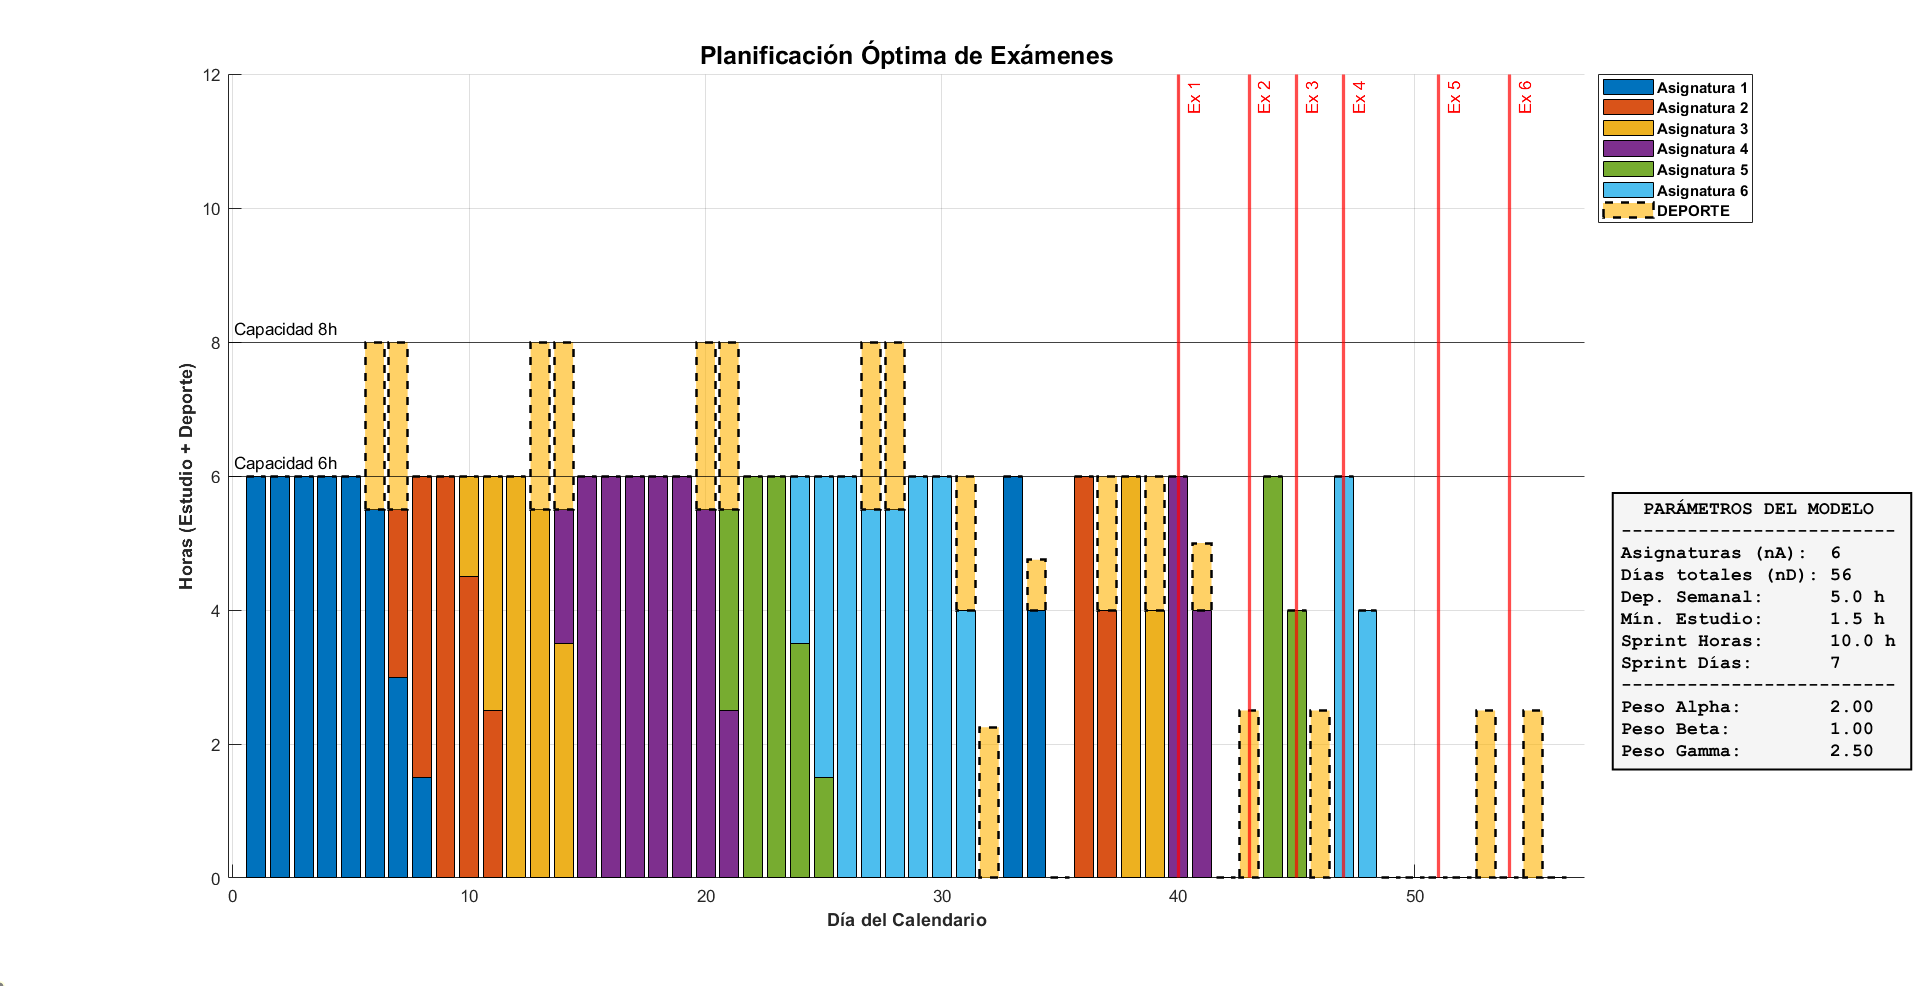
\includegraphics[width=0.75\linewidth]{FIGURA_3.png}
        \caption{Calendario académico; saturación del descanso}
        \label{fig:placeholder}
    \end{figure}
\end{itemize}

\subsubsection{Análisis de la lógica binaria (bloques mínimos)}

En todas las gráficas de este experimento se aprecia que no existen sesiones de estudio residuales (de pocos minutos). El uso de las variables binarias $y_{a,d}$ obliga al modelo a crear bloques de al menos 1.5h, lo que garantiza que el calendario resultante sea realista y productivo para un estudiante, evitando el ``ruido'' de asignaciones temporales insignificantes.

\subsection{Experimento II: Calendario real de exámenes}

Tras validar el modelo con escenarios genéricos, se ha sometido al sistema a una prueba con nuestro calendario académico real de esta evaluación (Ingeniería en Inteligencia Artificial (2.º curso, 2.º trimestre) — Tecnun). Este escenario es especialmente complejo debido a la proximidad entre los exámenes y la diversidad de las materias (horas necesarias para cada una dependiendo de los créditos y horas ya cursadas): Data Analytics, Machine Learning, Física Computacional, Visualización de Datos, Técnicas de Optimización IA y Estructura de Datos.

\begin{figure}[H]
    \centering
    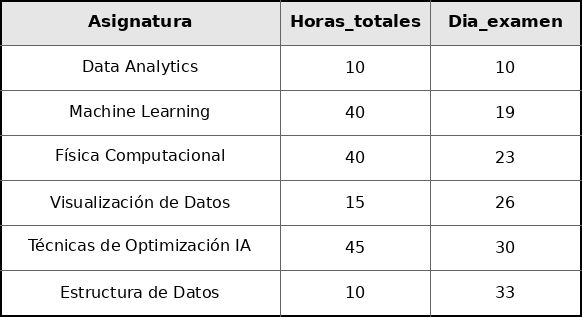
\includegraphics[width=0.65\linewidth]{Code_Generated_Image (2).png}
    \caption{Tabla de asignaturas, Experimento II}
    \label{fig:placeholder}
\end{figure}

\subsubsection{Gestión de la saturación por proximidad de fechas}

A diferencia de los experimentos anteriores de 56 días, aquí el horizonte es mucho más corto (33 días). A pesar de esto, se observa cómo el modelo soluciona correctamente los días más intensos (especialmente entre los días 20 y 30, donde se concentran 4 exámenes).

\begin{figure}[H]
    \centering
    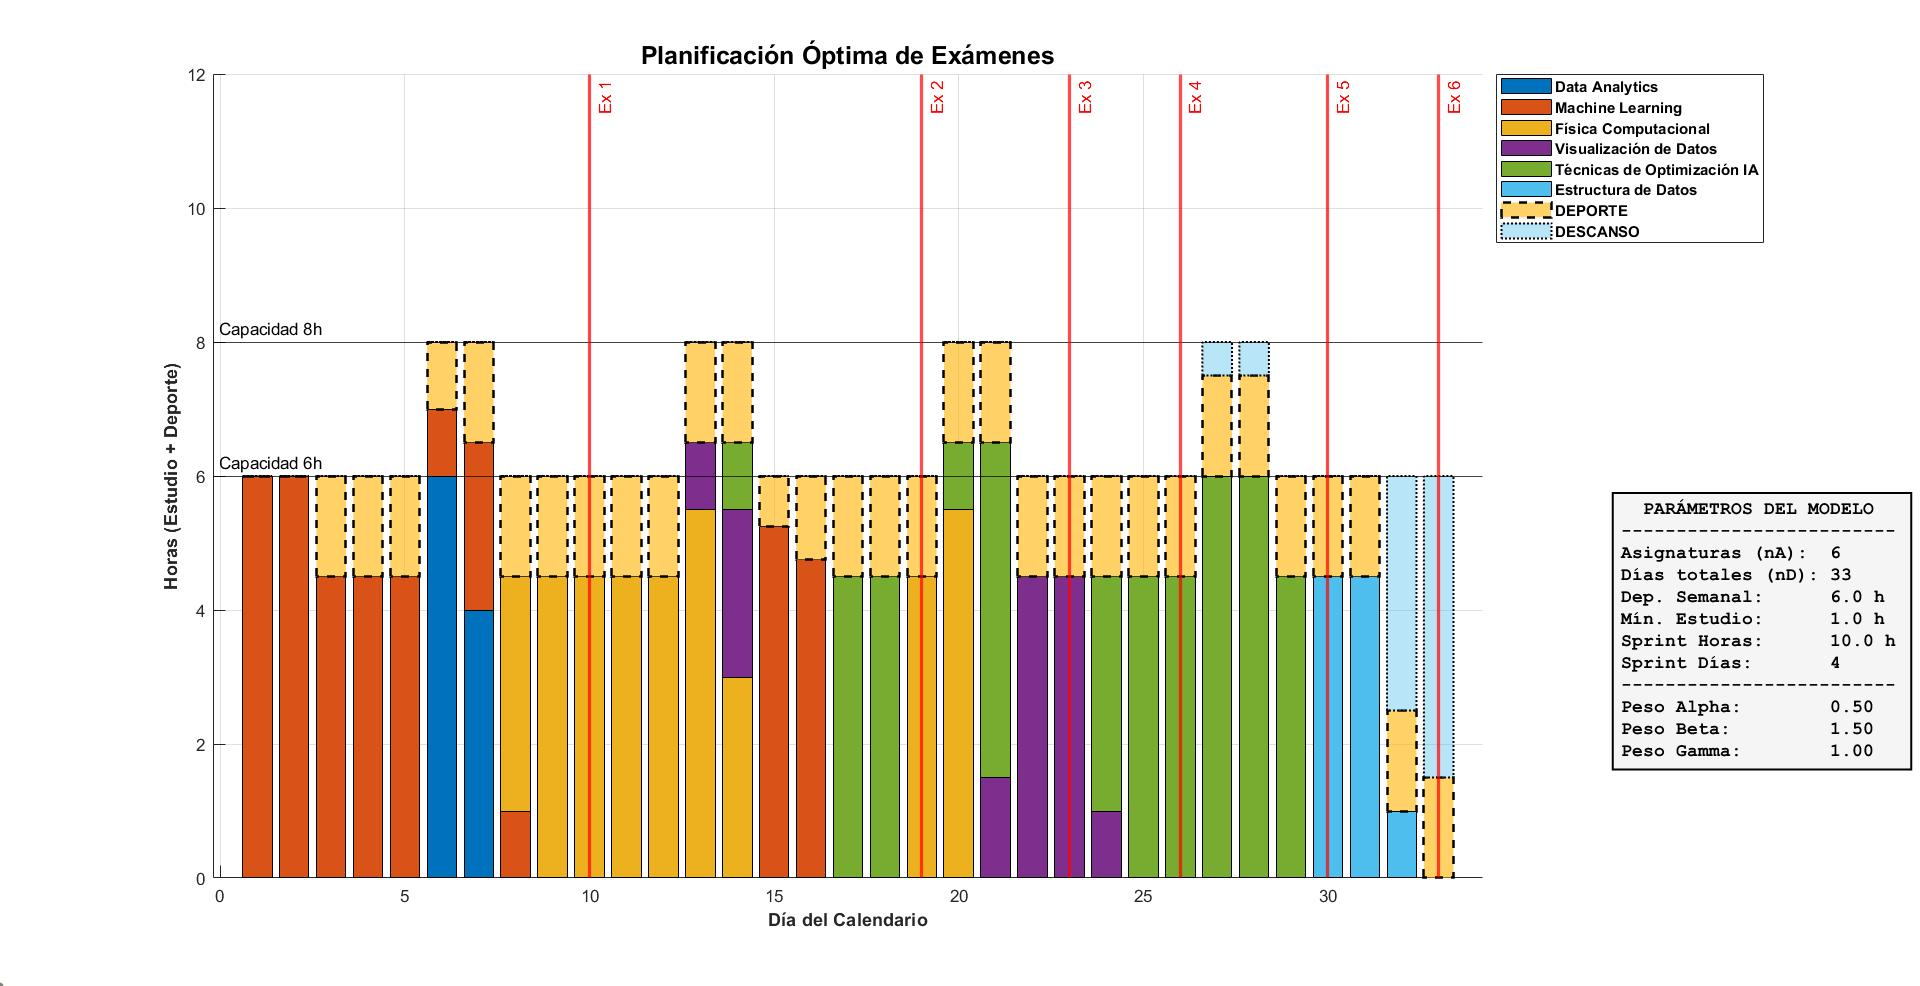
\includegraphics[width=0.75\linewidth]{Prueba_Real_FIG.jpg}
    \caption{Calendario académico; caso real, Experimento II}
    \label{fig:placeholder}
\end{figure}

\textbf{Comportamiento observado:} El sistema adelanta la carga de Data Analytics y Machine Learning (los primeros 2 exámenes) a la primera semana para liberar capacidad de cara a los exámenes finales, demostrando una buena gestión de recursos que evita el colapso en la recta final.

\subsubsection{Flexibilidad en la capacidad diaria y uso del descanso}

En este escenario, se han ajustado los pesos a valores más equilibrados ($\beta = 1.50$ y $\gamma = 1.00$).

Se aprecia que el modelo utiliza el descanso de forma estratégica en los últimos días (días 30--33). Una vez superado el pico de exámenes de las asignaturas 4 y 5, el modelo detecta que puede cumplir con la última asignatura sin sacrificar el bienestar, permitiendo periodos de inactividad que reducen el estrés.

\subsubsection{Adaptación del Sprint Final en un entorno real}

Con un parámetro de \textit{Sprint Horas} de 10.0h en solo 4 días, el modelo se ve obligado a saturar la capacidad hasta las 8h en los fines de semana previos a los exámenes de Física Computacional y Estructura de Datos.

Es notable cómo, a pesar de la exigencia, el sistema logra encajar diariamente los bloques de deporte (barras amarillas), cumpliendo con el mínimo semanal de 6.0h. Esto valida que el modelo es capaz de encontrar soluciones de bienestar incluso en periodos de máximo estrés académico.

\subsubsection{Conclusiones del Experimento II}

El resultado de la prueba real confirma que el sistema de indexación lineal y la lógica de penalización por procrastinación funcionan en entornos de alta densidad de tareas. El plan generado no solo es factible desde el punto de vista de las horas, sino que es coherente al priorizar materias según su dificultad y fecha de evaluación.
\end{document}